\documentclass{article}
\usepackage{graphicx}
\usepackage{geometry}
\usepackage{amsmath}
\usepackage{float}
\usepackage{bm}
\usepackage{fontspec}
\usepackage{amsfonts}
\usepackage{booktabs}
% \setmainfont{Calibri} %字体
% \usepackage[UTF8]{ctex} %中文包
\usepackage{xcolor}
\geometry{a4paper,scale=0.8}

\begin{document}
In our previous work titled " Topological Quantization of Superfluid Stiffness in Dirac Materials", we demonstrated the mechanism of the quantization of the superfluid stiffness in Dirac materials. Our findings revealed that the superfluid stiffness in Dirac materials remains quantized as long as the number of Berry monopoles is conserved in the synthetic space. Specifically, in the case of charge-neutral and Zeeman field neutral conditions, the superfluid stiffness($ D_{\textrm{total}}  $) is equal to $  \frac{\Delta}{\pi}  $  per cone (we will derive a more general $ D_{\textrm{total}} $ later ). Therefore the quantity of superfluid stiffness is determined by the number of Dirac cones present. This raises a intriguing question: can we establish a mapping from the value of superfluid stiffness to the number of Dirac cones? Such a mapping would have practical implication allowing experimentalists to determine the number of Dirac cones by measuring the superfluid stiffness of real materials, like graphene.

In this note, we aim to address above question through a supervised machine learning approach. We train our neural network by feeding superfluid stiffness data obtained from the Dirac model that may encompass higher order Dirac cones, enabling it to predict the Hamiltonian's total absolute vorticity. The total absolute vorticity is equal to the number of Dirac cones times their corresponding order.  After fully training our network, we test our model's performance using superfluid stiffness data for graphene which is a 2D material. Our model achieve a high accuracy, which validates the effectiveness of our method.

\section{Dirac model and higher order band touching points}
In this section, we will introduce the Dirac model and derive the corresponding superfluid stiffness. It's important to note that we utilize Dirac model's superfluid stiffness as input for our neural network during training process.

The Hamiltonian of the Dirac model in momentum space can be written as 
\begin{align}
    \hat{h} &= \left(a k_x + ib k_y\right)^n \hat{\sigma}_+ + \left(a k_x - ib k_y\right)^n \hat{\sigma}_- + \mu \\
            &= |\widetilde{k}|^n \cos(n \theta) \hat{\sigma}_x - |\widetilde{k}|^n \sin(n \theta) \hat{\sigma}_y + \mu\\
            &= |\widetilde{k}|^n e^{in \theta \hat{\sigma}_z}\hat{\sigma}_x + \mu,  
\end{align}
where $ \mu $ is chemical potential, $ n $ is a positive integer, $ \hat{\sigma} $ denote Pauli matrices in sub-lattice space, $ |\widetilde{k}|= \sqrt{(a k_x)^2 + (b k_y)^2 }   $ and $ \tan(n \theta) = \frac{(ak_x-ibk_y)^n}{(ak_x+ibk_y)^n} $. The eigen-vector of the Hamiltonian is read as 
\begin{align}
    |u_\pm\rangle = \frac{1}{\sqrt{2} } \left(\begin{array}{c}
         1 \\
         \pm e^{-in \theta} \\
    \end{array}\right),
\end{align}
whose corresponding eigen-value is presented as $ \epsilon_{\pm} = \pm |\widetilde{k}|^n + \mu   $. 

Now let's consider that superconductivity is introduced into the system. The super current flow in the direction of gradient of superconducting phase $ \phi $ proportional to superfluid stiffness, such as $ J_{i}=D_{ij}\nabla_i \phi$, where superfluid stiffness $ D $ is a symmetric matrix
\begin{align}
    D & = \left(\begin{array}{cc}
        D_{xx}  & D_{xy}    \\
        D_{yx}  & D_{yy}   \\
    \end{array}\right)
\end{align}
The element of superfluid stiffness can be read as:
\begin{align}
    D_{ij} = 2\Delta^2 \iint \frac{dk_x}{2\pi} \frac{dk_y}{2\pi} \sum_{\alpha,\beta=\pm} \frac{\langle u_{\alpha}|\partial_{i} \hat{h}|u_{\beta}\rangle\langle u_{\beta}|\partial_{j} \hat{h}|u_{\alpha}\rangle}{E_\alpha^2 - E_\beta^2} \left(\frac{f(E_\beta)}{E_\beta} - \frac{f(E_\alpha)}{E_\alpha} \right),\label{eq:SS}
\end{align} 
where $ i,j \in \{x,y\} $, $ f(E) = \Theta(B+E)-\Theta(B-E)=\Theta(E-\left\vert B \right\vert ) $ and $ E_\pm = \sqrt{\epsilon_\pm^2 + \Delta^2}  $. Utilizing Eq. (\ref{eq:SS}), we immediately obtain the superfluid stiffness of the Dirac model,
\begin{align}
    D_{xx}  &=\frac{a}{b} (D_{\textrm{intra}} + D_{\textrm{inter}}),\\ \label{eq:Dxx }
    D_{yy}  &=\frac{b}{a} (D_{\textrm{intra}} + D_{\textrm{inter}}),\\ \label{eq:Dyy }
    D_{xy} &= D_{yx} = 0,
\end{align}
where
\begin{align*}
    D_{\textrm{intra}} &=  n \frac{\sqrt{\mu^2+\Delta^2}}{2\pi}\Bigg\{ \Theta(|\Delta|-|B|)+\Theta(|B|-|\Delta|)\Theta(\sqrt{\mu^2+\Delta^2}-|B|) \bigg[1-\frac{|\mu|}{\sqrt{\mu^2+\Delta^2}}\frac{|B|}{\sqrt{B^2-\Delta^2}}\bigg]\Bigg\},\\
    D_{\textrm{inter}} &= \frac{n}{|\mu|}\frac{\Delta^2}{2\pi} \Bigg\{ \Theta(|\Delta|-|B|)\ln(\frac{\sqrt{\mu^2+\Delta^2}+|\mu|}{|\Delta|})+\Theta(|B|-|\Delta|)\Theta(\sqrt{\mu^2+\Delta^2}-|B|)\ln(\frac{\sqrt{\mu^2+\Delta^2}+|\mu|}{\sqrt{B^2-\Delta^2}+|B|}) \Bigg\}.    
\end{align*}
when $\mu \to 0$, $D_{\textrm{inter}}=n\frac{|\Delta|}{2\pi}\Theta(|\Delta|-|B|) $. For zero Zeeman field and chemical potential, $ D_{xx}=D_{yy} = n \frac{\left\vert \Delta \right\vert}{\pi}     $ which aligns in our initial statement. 

In  order to eliminate the effect of anisotropy, we are interested at the determinant of superfluid stiffness 
\begin{align}
    \left\vert D \right\vert &= D_{xx}D_{yy} - D{xy}D{yx}\label{eq:D}\\
                             &= D_{\textrm{total}}^2, 
\end{align}
which does not include $ a,b $.  Here $ D_{\textrm{total}} = D_{\textrm{intra}} + D_{\textrm{inter}} $. By considering the determinant, we can effectively capture the overall behavior and characteristics of the superfluid stiffness, while cancels the influence of the inherent anisotropy present in the system. 
It is worth to notice that $ |D|=D_{\textrm{total}}^2  $ appears because of $ D_{xy}= D_{yz} = 0   $ in Dirac model, for more general case we need to calculate  Eq. (\ref{eq:D}). For convenience, in the following discussion we set $ \Delta = 1 $. Figure. (\ref{fig: Deter_D_3D}) illuminates the amplitude of $ |D| $ with $ mu $ and $ B $ varying in the range of $ \left(-3,3\right) $. Notably,one may observe that $ |D| $ changes discontinuously at $ |B| = \Delta $, specifically when $ mu=0 $ $ |D| $ experiences an abrupt drop $ \frac{1}{\pi^2} $ (see inset figure). This discontinuity may serves as an crucial signal in identifying the so called total absolute vorticity. 

\begin{figure}[H]
    \centering
    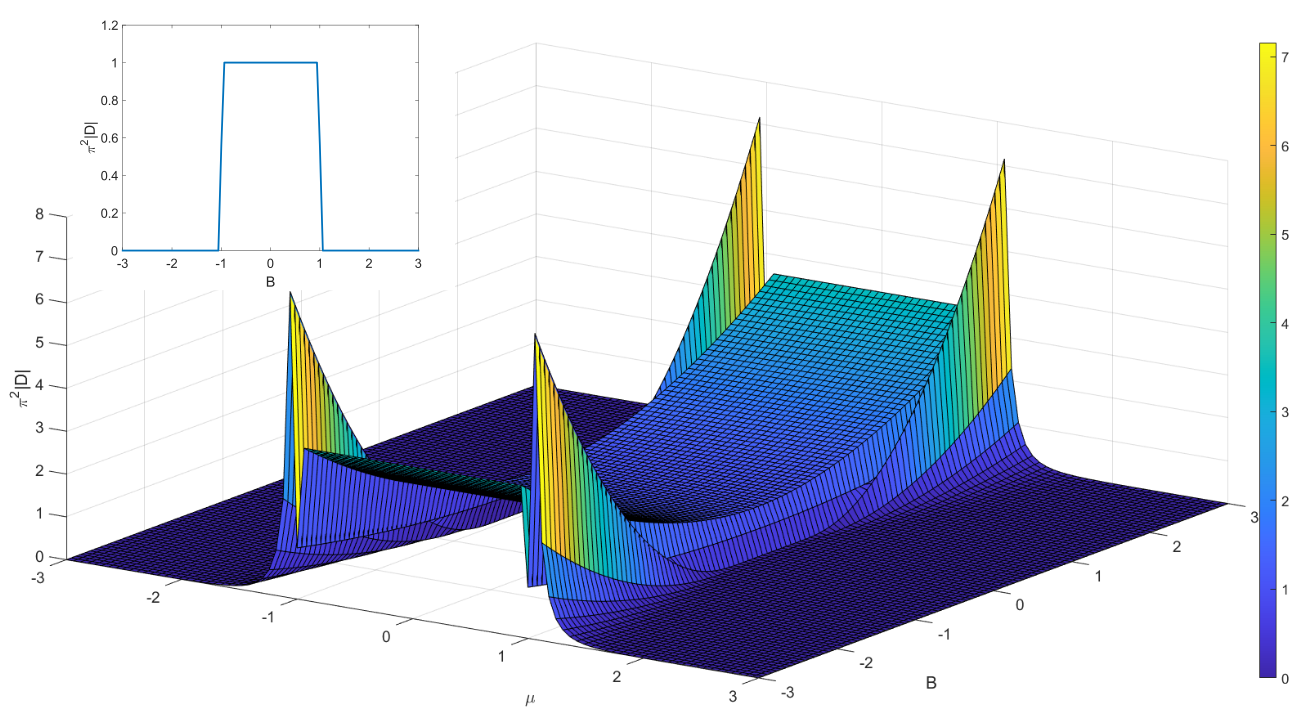
\includegraphics[width=0.8\textwidth]{matlab code/D_deter_3D_hybrid.pdf}
    \caption{Amplitude of $ |D| $ with $ mu $ and $ B $ varying in the range of $ \left(-3,3\right) $. Inset figure shows variation of $ |D| $ with $ B $ varying and $ mu =0 $. }
    \label{fig: Deter_D_3D}
\end{figure}

\subsection{Total absolute vorticity}
The total absolute vorticity is equal to the number of Dirac cones times their corresponding order, which is our neural network's main prediction. One can rewrite above Dirac model Hamiltonian as a vector form 
\begin{align}
    \hat{h} &= \mathbf{H} \cdot \bm{\sigma},
\end{align}
where $ \mathbf{H}= \left(|\widetilde{k}|^n \cos(n \theta),|\widetilde{k}|^n \sin(n \theta) \right) $. The angle of vector $ \mathbf{H} $ is denoted by $ \phi = \arctan(-\tan(n \theta)) = -n \theta $. The total absolute vorticity is written as 
\begin{align}
    w &= \frac{1}{2\pi}\left\vert \oint d \phi  \right\vert =  n. 
\end{align}

\section{Parabolic model}
In previous section, we compute the contribution of a single Dirac cone to superfluid stiffness. In this section, we study the contribution of a trivial crossing point of the Fermi level to the superfluid stiffness. Without loss generality, we study the parabolic model whose Hamiltonian can be written as 
\begin{align}
    \hat{h}_{\textrm{p}} &= \left[(a k_x)^2 + (b k_y)^2\right] \hat{\sigma}_x + \mu 
\end{align}
whose eigen-vectors are 
\begin{align}
    u^{\textrm{p}} _\pm &= \left(\begin{array}{c}
         1 \\
         \pm 1 \\
    \end{array}\right)
\end{align}
corresponds to eigen-value $\epsilon^{\textrm{p}}_\pm =  \pm |\widetilde{k}|^2 + \mu  $. Applying Eq. (\ref{eq:SS}), the contribution to the superfluid stiffness is 
\begin{align}
    D^{\textrm{p}} _{xx} &= \frac{a}{b}D_{\textrm{intra}}, \\   
    D^{\textrm{p}} _{yy} &= \frac{b}{a}D_{\textrm{intra}}, \\   
    D^{\textrm{p}} _{xy} &= D^{\textrm{p}}_{yx} =0. 
\end{align}
For trivial case, the interband part of superfluid stiffness is equal to zero. 

Since the parabolic model's Hamiltonian only have contribution to $ \hat{\sigma}_x $, then the corresponding vorticity is equal to zero. 

\section{Training data set}
Before constructing the input data set, it's important to emphasize the primary objective of our neural network. Our neural network aims to predict two key aspects: firstly, whether the crossing point of the Fermi level corresponds to a Dirac cone. Secondly, the number of Dirac cones within a small window as the parameters $ B $ and $ \mu $ vary.

To achieve this goal, we begin by selecting a interested central chemical potential, denoted as $ \mu_0 $ which serves as the reference point. And then compute the determinant of the superfluid stiffness within a defined window varying $ \mu $ in the range of $ \left(\mu_0 - \mu_{\textrm{off}},\mu_0+ \mu_{\textrm{off} }   \right)$ and $ B $ in $ \left(-B_{\textrm{off}},B_{\textrm{off}}  \right) $. Finally, a matrix labeled by the total absolute vorticity is obtained. By varying the central potential and total absolute vorticity, we can generate a set of labeled matrices that serve as the input data for our neural network. Each labeled matrix corresponds to a different combination of total absolute vorticity and central chemical potential. Fig. (\ref{fig: Training Data}) shows a example of training data.

\begin{figure}[H]
    \centering
    \includegraphics[width=1\textwidth]{Training Data.pdf}
    \caption{Training data set example. The first row illustrates the determinant of superfluid stiffness for a parabolic model with $ \mu_0 $ varying in the range of $ \left(-3,3\right) $, $  \mu_{\textrm{off}} = B_{\textrm{off}} = 2$  . The second row represents the determinant for a Dirac model($ n=1 $) where $ \mu_0 $ varies in the same range. The corresponding vorticity is shown above the matrix.}
    \label{fig: Training Data}
\end{figure}

\section{Graphene model}
The Hamiltonian of Graphene in momentum space can be written as 
\begin{align}
    \hat{h}_{\textrm{g}} = &-t \left[\cos(\frac{1}{2}k_x + \frac{\sqrt{3}}{2} k_y )+ \cos(\frac{1}{2}k_x - \frac{\sqrt{3}}{2} k_{y}  )+ \cos(-k_x)\right] \hat{\sigma}_x \nonumber\\
    &-t \left[\sin(\frac{1}{2}k_x + \frac{\sqrt{3}}{2} k_y )+ \sin(\frac{1}{2}k_x - \frac{\sqrt{3}}{2} k_y )+ \sin(-k_x)\right] \hat{\sigma}_y+\mu,
\end{align}
where $ t \approx 2.8eV $ is hopping amplitude. 

The eigen-energy have formula $ \epsilon^{\textrm{g}}_\pm = \pm t \sqrt{3+2 \cos(\sqrt{3} k_y )+4 \cos(\frac{\sqrt{3}}{2}k_y ) \cos(\frac{3}{2}k_x)} + \mu  $ and its corresponding eigen-vector can be read as 
\begin{align}
    u^{\textrm{g}}_\pm = \frac{1}{\sqrt{2} } \left(\begin{array}{c}
         1 \\
         \pm i e^{i \theta_{\textrm{g}} } \\
    \end{array}\right),
\end{align}
where
\begin{align}
    \tan(\theta_{\textrm{g}} ) &= \frac{\sin(\frac{1}{2}k_x + \frac{\sqrt{3}}{2} k_y )+ \sin(\frac{1}{2}k_x - \frac{\sqrt{3}}{2} k_y )+ \sin(-k_x)}{\cos(\frac{1}{2}k_x + \frac{\sqrt{3}}{2} k_y )+ \cos(\frac{1}{2}k_x - \frac{\sqrt{3}}{2} k_{y}  )+ \cos(-k_x)} 
\end{align}
Applying Eq. (\ref{eq:SS}), one obtain the determinant of graphene's superfluid stiffness. 

\subsection{Total absolute vorticity of graphene}
Since the hopping amplitude is much larger than the induced superconductivity in graphene $ \Delta \approx 1meV $, the Hamiltonian can be approximately described by two Dirac cones 
\begin{align}
    \hat{h}_{\textrm{g}} &\approx   v_{F} \left( q_x \hat{\sigma}_x + q_y \hat{\rho}_z \hat{\sigma}_y \right),
\end{align}
where $ \mathbf{q} $ is the momentum measured relatively to the Dirac points, $ v_F $ is the Fermi velocity, given by $ v_F = \frac{3}{2} t $, $ \hat{\rho} $ are Pauli matrices in valley space. 

The total absolute vorticity is the sum of absolute vorticity of two containing Dirac cones, i.e. $ w_{\textrm{g}} \approx 2  $. The determinant of graphene would be labeled as $ 2 $ if Dirac cones present within the defined window, else would be labeled as $ 0 $. By varying hopping amplitude and central chemical potential, one gather a set of test date.

\section{Neural network}
The neural network work flow and the structure is shown in Fig. (\ref{fig: Neural network}). One input the determinant of superfluid stiffness to the neural network which output the total absolute vorticity. The neural network encompass two convolutional layers with 32 channels of kernel size $ 3 \times 3 $ and 2 channels of kernel size $ 3 \times 3 $, followed by two fully connected layers with the first one containing 1024 neurons and the second 512 neurons. At last, the neural network output the total absolute vorticity. 
\begin{figure}[H]
    \centering
    \includegraphics[width=1\textwidth]{Neural network.pdf}
    \caption{Schematic of the machine learning workflow and the structure of the convolutional neural network.}
    \label{fig: Neural network}
\end{figure}

We split the Dirac and parabolic model data set into 2 part, 4000 determinant samples with the total absolute vorticity $ w \in \left(0,6\right) $, randomly choose $ 70\% $ of them for training data set and the remainder as (i) the first validation data set which was not used during training process; 1000 samples with the total absolute vorticity $ w \in \left(7,9\right) $ (ii) as the second validation data set whose vorticity is unseen in training process. (iii) Meanwhile we generate 4000 determinant samples from graphene with $ t \in \left(2000,4000\right) $ as test data set. The test result is presented in Table (\ref{tab:Performance}).

\begin{table}[H]
    \centering
    \begin{tabular}{c|c|c|c}
        \toprule
             & Validation(i)  & Validation(ii) & Test(iii)   \\
        \midrule
        Accuracy     & 100\% & 98.3\% &  98.0\%  \\
        \bottomrule
    \end{tabular}
    \caption{Performance of the neural network with respect to different validation and test data sets.}
    \label{tab:Performance}
\end{table}
\end{document}

